\documentclass{article}

\usepackage{amsmath}
\usepackage{amssymb}
\usepackage{mathtools}
\usepackage{fullpage}
\usepackage[T1]{fontenc}
\usepackage{lmodern}
\usepackage{tikz}
\usetikzlibrary{calc,intersections,through,backgrounds}
\usetikzlibrary{bayesnet}
\usepackage{tikzscale}
\usepackage{tkz-euclide}
\usepackage{tcolorbox}
\tcbuselibrary{skins,breakable}
% pgfplots
\usepackage{pgfplots}
\pgfplotsset{compat=1.8}
% For entities in pgfplots
\newcommand{\entpgf}[1]{\texttt{#1}}

\begin{document}

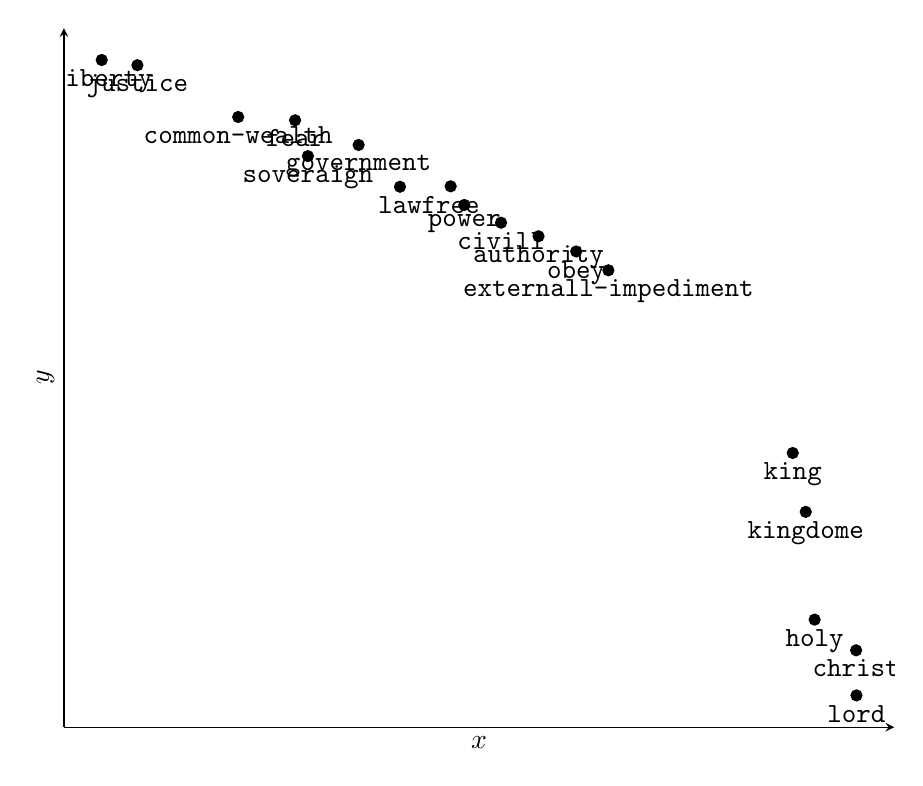
\begin{tikzpicture}
\pgfplotsset{ticks=none}
		\begin{axis}[
		    axis x line=bottom,
			axis y line=left,
			xmin=-6.813135-0.40458216667175295, xmax=1.2785078+0.40458216667175295,
			ymin=-10.181688-0.6951928615570069, ymax=3.7221692+0.6951928615570069,
			xtick={-6.813135,1.2785078},ytick={-10.181688,3.7221692},
			xlabel=$x$,ylabel=$y$,
			%x label style={anchor=west},
			%y label style={anchor=south},
			width=\textwidth
			]
			\addplot+[mark options={fill=black,color=black},only marks,point meta=explicit symbolic, nodes near coords] coordinates {
(-2.130077362060547, -0.13540464639663696)[]
(1.2746942043304443, -9.194621086120605)[]
(-2.5317118167877197, 0.16266223788261414)[]
(-5.35002326965332, 2.4747960567474365)[]
(-1.381063461303711, -0.879364013671875)[]
(-4.739980697631836, 2.4027860164642334)[]
(-3.0720303058624268, 0.9579295516014099)[]
(-4.058857440948486, 1.862748146057129)[]
(0.8299546241760254, -8.523327827453613)[]
(-6.430646896362305, 3.608384847640991)[]
(0.5951986312866211, -4.877157211303711)[]
(0.7346023321151733, -6.165247917175293)[]
(-3.615633249282837, 0.9484952688217163)[]
(-6.813135147094727, 3.7221691608428955)[]
(1.2785078287124634, -10.18168830871582)[]
(-1.7261645793914795, -0.4675861895084381)[]
(-2.9259326457977295, 0.5500147342681885)[]
(-4.602591037750244, 1.6189823150634766)[]
};
\node (authority) at (axis cs:-2.1300774, -0.13540465){};
\node (christ) at (axis cs:1.2746942, -9.194621){};
\node (civill) at (axis cs:-2.5317118, 0.16266224){};
\node (common-wealth) at (axis cs:-5.3500233, 2.474796){};
\node (externall-impediment) at (axis cs:-1.3810635, -0.879364){};
\node (fear) at (axis cs:-4.7399807, 2.402786){};
\node (free) at (axis cs:-3.0720303, 0.95792955){};
\node (government) at (axis cs:-4.0588574, 1.8627481){};
\node (holy) at (axis cs:0.8299546, -8.523328){};
\node (justice) at (axis cs:-6.430647, 3.6083848){};
\node (king) at (axis cs:0.59519863, -4.877157){};
\node (kingdome) at (axis cs:0.73460233, -6.165248){};
\node (law) at (axis cs:-3.6156332, 0.94849527){};
\node (liberty) at (axis cs:-6.813135, 3.7221692){};
\node (lord) at (axis cs:1.2785078, -10.181688){};
\node (obey) at (axis cs:-1.7261646, -0.4675862){};
\node (power) at (axis cs:-2.9259326, 0.55001473){};
\node (soveraign) at (axis cs:-4.602591, 1.6189823){};
\node[anchor = north, xshift=0.0, yshift=0.0] (authorityl) at(axis cs: -2.1300774, -0.13540465){$\entpgf{authority}$};
\node[anchor = north, xshift=0.0, yshift=0.0] (christl) at(axis cs: 1.2746942, -9.194621){$\entpgf{christ}$};
\node[anchor = north, xshift=0.0, yshift=0.0] (civilll) at(axis cs: -2.5317118, 0.16266224){$\entpgf{civill}$};
\node[anchor = north, xshift=0.0, yshift=0.0] (common-wealthl) at(axis cs: -5.3500233, 2.474796){$\entpgf{common-wealth}$};
\node[anchor = north, xshift=0.0, yshift=0.0] (externall-impedimentl) at(axis cs: -1.3810635, -0.879364){$\entpgf{externall-impediment}$};
\node[anchor = north, xshift=0.0, yshift=0.0] (fearl) at(axis cs: -4.7399807, 2.402786){$\entpgf{fear}$};
\node[anchor = north, xshift=0.0, yshift=0.0] (freel) at(axis cs: -3.0720303, 0.95792955){$\entpgf{free}$};
\node[anchor = north, xshift=0.0, yshift=0.0] (governmentl) at(axis cs: -4.0588574, 1.8627481){$\entpgf{government}$};
\node[anchor = north, xshift=0.0, yshift=0.0] (holyl) at(axis cs: 0.8299546, -8.523328){$\entpgf{holy}$};
\node[anchor = north, xshift=0.0, yshift=0.0] (justicel) at(axis cs: -6.430647, 3.6083848){$\entpgf{justice}$};
\node[anchor = north, xshift=0.0, yshift=0.0] (kingl) at(axis cs: 0.59519863, -4.877157){$\entpgf{king}$};
\node[anchor = north, xshift=0.0, yshift=0.0] (kingdomel) at(axis cs: 0.73460233, -6.165248){$\entpgf{kingdome}$};
\node[anchor = north, xshift=0.0, yshift=0.0] (lawl) at(axis cs: -3.6156332, 0.94849527){$\entpgf{law}$};
\node[anchor = north, xshift=0.0, yshift=0.0] (libertyl) at(axis cs: -6.813135, 3.7221692){$\entpgf{liberty}$};
\node[anchor = north, xshift=0.0, yshift=0.0] (lordl) at(axis cs: 1.2785078, -10.181688){$\entpgf{lord}$};
\node[anchor = north, xshift=0.0, yshift=0.0] (obeyl) at(axis cs: -1.7261646, -0.4675862){$\entpgf{obey}$};
\node[anchor = north, xshift=0.0, yshift=0.0] (powerl) at(axis cs: -2.9259326, 0.55001473){$\entpgf{power}$};
\node[anchor = north, xshift=0.0, yshift=0.0] (soveraignl) at(axis cs: -4.602591, 1.6189823){$\entpgf{soveraign}$};

\end{axis}
\end{tikzpicture}

\end{document}